\documentclass[../main.tex]{subfiles}

\begin{document}

高偏差: 模型具有很强的(错误的)先验知识(偏见)

高方差: 模型过于依赖训练数据

高偏差+高方差: 即有很强的先验知识, 又过于依赖数据

\begin{figure}
    \centering
    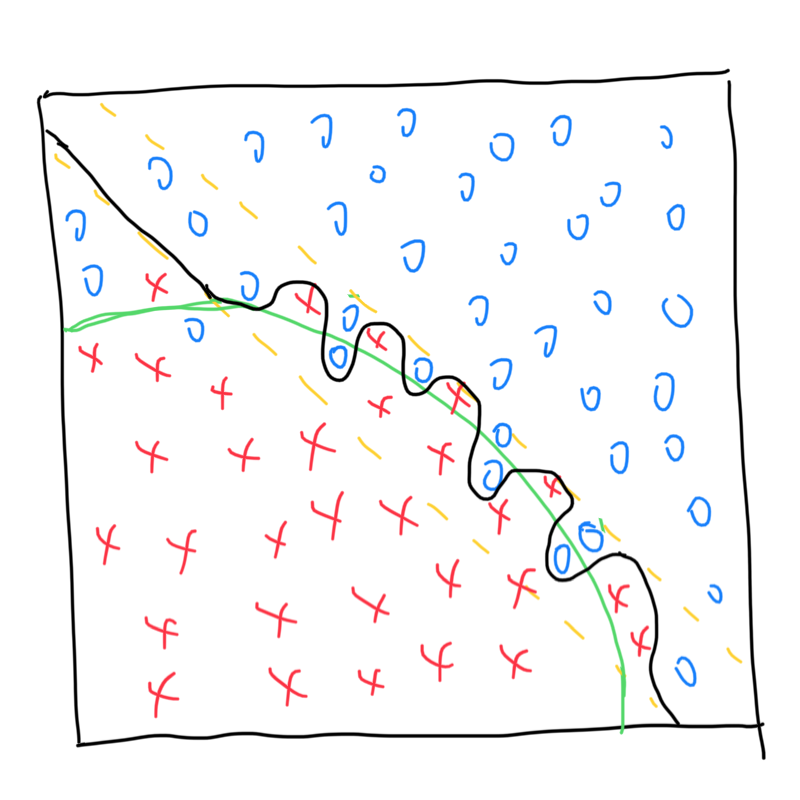
\includegraphics[width=.6\textwidth]{../figure/2-8.png}
    \caption{高偏差+高方差}
    \label{img2-8}
\end{figure}

如图\ref{img2-8}所示, 该图描述了一个二分类问题.
其中, 红X和蓝O是需区分的两类, 绿色的曲线为理想的决策曲线,
黄色的线段为人为规定的决策区域(模型只能在其中进行决策),
黑线为模型最终训练得到的决策曲线.
在这个模型中, 人为规定的决策区域给模型提供了一个很强的先验(偏见),
而模型在其中又过分拟合每个训练数据.
最终, 得到了一个高偏差+高方差的模型.

\end{document}